% chapter 1 section 2

\section{能量与动量}

\subsection{能量}
\label{subsec:能量}

\subsubsection{功与功率}

倘若物体在力F的作用下运动了s距离,则说该力对物体做了功,日文为仕事,其单位是$J=N\cdot m$。即功是\underline{力在运动方向上随距离的累积}。其严格定义是力与位移的标量积。
\begin{figure}[ht!]
    \centering
    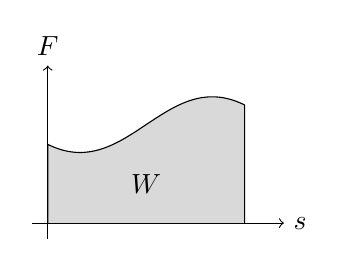
\begin{tikzpicture}
        \draw[->] (-0.2, 0) -- (3, 0) node[right] {$s$};
        \draw[->] (0, -0.2) -- (0, 2) node[above] {$F$};
        \filldraw[color=black, fill=gray, fill opacity=0.3] (0, 0) -- 
            (0, 1) .. controls (1, 0.5) and (1.5, 2) .. (2.5, 1.5) -- (2.5, 0);
        \node at (1.25, 0.5) {$W$};
    \end{tikzpicture}
    \caption{$F-s$图像与功}
\end{figure}
如果物体能对外做功,便说该物体具有能量。
\begin{itembox}[l]{功}
    \begin{equation*}
        W=\vec{F}\cdot\vec{s}=Fs\cos\theta
    \end{equation*}
    \begin{itemize}
        \item 可正可负,取决于位移的方向
        \item 力与位移方向垂直时不做功,$W=0$
    \end{itemize}
\end{itembox}
此外,类比于距离与速度的关系,单位时间内所做的功称为功率,日文为仕事率,其单位是$W=J/s$。处理问题时除了定义式,也常用$P=\frac{W}{t}=\frac{\vec{F}\cdot\vec{s}}{t}=\vec{F}\cdot\vec{v}$。

\subsubsection{动能}

日文为運動エネルギー,专指\underline{运动中}的物体具有的能量。
\begin{itembox}[l]{动能}
    \begin{equation*}
        E_k=\frac12mv^2
    \end{equation*}
\end{itembox}
如图所示,在光滑水平面上,质量为m的物体受恒力F作用运动了s距离。
\begin{figure}[ht!]
    \centering
    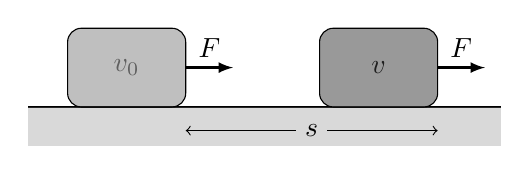
\begin{tikzpicture}
        \draw (0, 0) -- (6, 0);
        \fill[fill=gray, opacity=0.3] (0, 0) rectangle (6, -0.5);
        \filldraw[color=black, fill=gray, fill opacity=0.5, rounded corners=5pt] (0.5, 0) rectangle node {$v_0$} (2, 1);
        \draw[thick, -latex] (2, 0.5) -- node[above] {$F$} (2.6, 0.5);
        \filldraw[color=black, fill=gray, fill opacity=0.8, rounded corners=5pt] (3.7, 0) rectangle node {$v$} (5.2, 1);
        \draw[thick, -latex] (5.2, 0.5) -- node[above] {$F$} (5.8, 0.5);
        \draw[<->] (2, -0.3) -- node[fill=gray!30] {$s$} (5.2, -0.3);
    \end{tikzpicture}
    \caption{动能定理}
\end{figure}
在此期间速度从$v_0$变化为了$v$。由牛二定律和运动学基本公式可得
\begin{equation*}
    W_{\textrm{外}}=Fs=mas=\frac12m(v^2-{v_0}^2)=\Delta E_k
\end{equation*}
即在这个过程中外力做功转化为了物体动能的增量。

\subsubsection{势能}

potential energy,日文为位置エネルギー。从英日双语着眼则可对“势”一字简做解析:势能这种能量是潜在的,并且是由物体\underline{位置状态}的改变激发。其具体定义为:物体从当前位置回到基准位置时保存力\footnote{做功与路径无关的力:重力、弹簧弹力、万有引力、电场力等}所做的功。

\begin{itembox}[l]{势能}
    \begin{itemize}
        \item 重力势能(重力による位置エネルギー):
        \begin{equation*}
            E_p=mgh
        \end{equation*}
        \item 弹力势能(弾性力による位置エネルギー):
        \begin{equation*}
            E_p=\frac12kx^2
        \end{equation*}    
    \end{itemize}
\end{itembox}

\subsubsection{机械能}

日文为力学的エネルギー,是动能与势能的统称,
\begin{itembox}[l]{机械能}
    \centering
    力学的エネルギー=運動エネルギー+位置エネルギー
\end{itembox}
在只有保存力做功或者非保存力不做功的情况下守恒。更一般的,因为系统内能量的总和始终一定,只是做了形式上的转化,所以对于非保存力参与的一般情况,可以采取如下两种思路处理问题。

\begin{itemize}
    \item 仅保存力参与:初始时总能量=终止时总能量
    \item 非保存力参与:终始总能量差额=消耗的能量
\end{itemize}

\subsection{动量}
\label{subsec:动量}

\subsubsection{动量与冲量}

\begin{figure}[ht!]
    \centering
    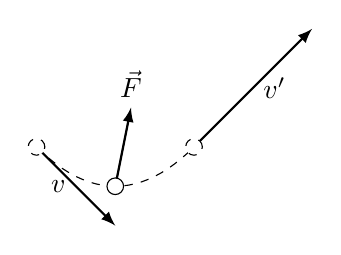
\begin{tikzpicture}
        \draw[dashed, domain=0:2] plot (\x, {0.5*(\x-1)^2-0.5});
        \draw[thick, -latex] (0, 0) -- node[left] {$v$} (1, -1);
        \draw[dashed, fill=white] (0, 0) circle (3pt);
        \draw[thick, -latex] (2, 0) -- node[right] {$v^\prime$} (3.5, 1.5);
        \draw[dashed, fill=white] (2, 0) circle (3pt);
        \draw[thick, -latex] (1, -0.5) -- (1.2, 0.5) node[above] {$\vec{F}$};
        \draw[fill=white] (1, -0.5) circle (3pt);
    \end{tikzpicture}
    \caption{动量与冲量}
\end{figure}
如图,对于质量为m的物体,在极短的时间t内施加一个力F,使其速度从$v$变为了$v^\prime$,观察其运动方程可知
\begin{gather*}
    \vec{F}=m\vec{a}=m\frac{\vec{v^\prime}-\vec{v}}{\Delta t}\\
    \vec{F}\Delta t=m\vec{v^\prime}-m\vec{v}
\end{gather*}
称其中$\vec{F}\Delta t$的部分为冲量,日文为力積,$m\vec{v}$的部分为动量,日文为運動量。由此可见,动量变化等于冲量\footnote{类比于功,可以说冲量是力在运动方向上随时间的累积}。

\subsubsection{动量守恒}

\begin{figure}[ht!]
    \centering
    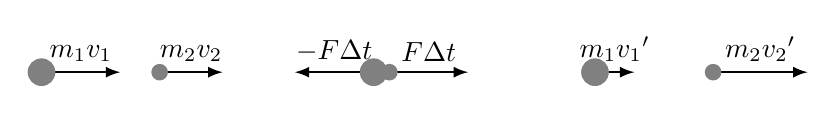
\begin{tikzpicture}
        \begin{scope}[xshift=-120]
            \draw[thick, -latex] (0, 0) -- node[above] {$m_1v_1$} ++ (1, 0);
            \fill[color=gray] (0, 0) circle (5pt);
            \draw[thick, -latex] (1.5, 0) -- node[above] {$m_2v_2$} ++ (0.8, 0);
            \fill[color=gray] (1.5, 0) circle (3pt);
        \end{scope}
        \begin{scope}
            \draw[thick, -latex] (0, 0) -- node[above] {$-F\Delta t$} ++ (-1, 0);
            \fill[color=gray] (0, 0) circle (5pt);
            \draw[thick, -latex] (0.2, 0) -- node[above] {$F\Delta t$} ++ (1, 0);
            \fill[color=gray] (0.2, 0) circle (3pt);
        \end{scope}
        \begin{scope}[xshift=80]
            \draw[thick, -latex] (0, 0) -- node[above] {$m_1{v_1}^\prime$} ++ (0.5, 0);
            \fill[color=gray] (0, 0) circle (5pt);
            \draw[thick, -latex] (1.5, 0) -- node[above] {$m_2{v_2}^\prime$} ++ (1.2, 0);
            \fill[color=gray] (1.5, 0) circle (3pt);
        \end{scope}
    \end{tikzpicture}
    \caption{动量守恒}
\end{figure}
对于上图的情形,根据牛三定律可得如下联立式:
\begin{equation*}
    \begin{cases}
        \vec{F}\cdot\Delta t&=m_2\vec{{v_2}^\prime}-m_2\vec{v_2}\\
        -\vec{F}\cdot\Delta t&=m_1\vec{{v_1}^\prime}-m_1\vec{v_1}
    \end{cases}
\end{equation*}
两侧相加整理后可得如下结论。
\begin{itembox}[l]{动量守恒}
    \begin{equation*}
        m_1\vec{v_1}+m_2\vec{v_2}=m_1\vec{{v_1}^\prime}+m_2\vec{{v_2}^\prime}
    \end{equation*}
\end{itembox}
其中左侧为碰撞前两物体的总动量,右侧为碰撞后两物体的总动量,因此在上述情形下动量守恒。

一般的,在由任意个物体组成的系统内,只要不受外力就都会满足动量守恒。而且根据动量的矢量性,其守恒也不局限于直线上,也可扩展到空间内。此时,即便有某一方向不满足条件,我们仍然可以列满足那个方向上的动量守恒。常见模型除了碰撞以外还有单个物体的分裂等。

\subsubsection{反弹系数}

日文为反発係数或者はねかえり係数,是一个描述两物体碰撞效果的数值。
\begin{itembox}[l]{反弹系数}
    \begin{equation*}
        e=-\frac{{v_1}^\prime-{v_2}^\prime}{v_1-v_2}\quad(0\le e\le1)
    \end{equation*}
    \begin{itemize}
        \item $e=0$:完全非弹性碰撞
        \item $0<e<1$:非弹性碰撞
        \item $e=1$:弹性碰撞(此时动能守恒)
    \end{itemize}
\end{itembox}
结合动量守恒公式可得两物体碰撞后速度的一般公式。
\begin{itembox}[l]{一般碰撞公式}
    \begin{equation*}
        \begin{cases}
            {v_1}^\prime=\frac{1}{m_1+m_2}(m_1v_1+m_2v_2-em_2(v_1-v_2))\\
            {v_2}^\prime=\frac{1}{m_1+m_2}(m_1v_1+m_2v_2+em_1(v_1-v_2))
        \end{cases}
    \end{equation*}
\end{itembox}

\subsubsection{特殊实例}

\paragraph{一动碰一静}即$v_2=0$的一般碰撞。此时一般碰撞公式会有所简化,而且两物体碰撞问题以此题型居多。
\begin{itembox}[l]{简化碰撞公式}
    \begin{equation*}
        \begin{cases}
            v_1=\frac{1}{m_1+m_2}(m_1-em_2)v\\
            v_2=\frac{1}{m_1+m_2}(m_1+em_1)v
		\end{cases}
    \end{equation*}
\end{itembox}

\paragraph{固定面碰撞}物体与墙面、地面等固定面碰撞的问题,其速度变化、高度变化十分具有代表性。
\begin{figure}[ht!]
    \centering
    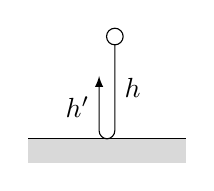
\begin{tikzpicture}
        \draw (0, 0) -- (2, 0);
        \fill[fill=gray, opacity=0.3] (0, 0) rectangle (2, -0.3);
        \draw[-latex, rounded corners=3pt] (1.1, 1.3) -- node[right] {$h$} (1.1, 0) -- (0.9, 0) -- node[left] {$h^\prime$} (0.9, 0.8);
        \draw[fill=white] (1.1, 1.3) circle (3pt);
    \end{tikzpicture}
    \caption{固定面碰撞}
\end{figure}
\begin{itembox}[l]{固定面碰撞结论}
    \begin{equation*}
        \begin{cases}
            v^\prime=ev\\
            h^\prime=e^2h
        \end{cases}
    \end{equation*}
\end{itembox}

\paragraph{斜向碰撞} 倘若物体从斜方向而来与平面发生碰撞,则需要利用运动的矢量性,将其分解处理。
\begin{figure}[ht!]
    \centering
    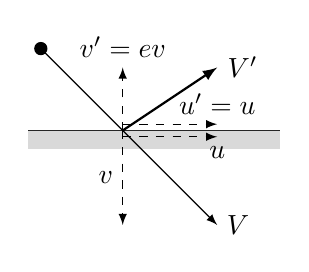
\begin{tikzpicture}[scale=0.8]
        \draw (0, 0) -- (4, 0);
        \fill[fill=gray, opacity=0.3] (0, 0) rectangle (4, -0.3);
        \fill (0.2, 1.3) circle (3pt);
        \draw[-latex] (0.2, 1.3) -- (3, -1.5) node[right] {$V$};
        \draw[dashed, -latex] (1.5, 0) -- node[left] {$v$} (1.5, -1.5);
        \draw[dashed, -latex] (1.5, -0.1) -- (3, -0.1) node[right, below] {$u$};
        \draw[dashed, -latex] (1.5, 0) -- (1.5, 1) node[above] {$v^\prime=ev$};
        \draw[dashed, -latex] (1.5, 0.1) -- (3, 0.1) node[right, above] {$u^\prime=u$};
        \draw[thick, -latex] (1.5, 0) -- (3, 1) node[right] {$V^\prime$};
    \end{tikzpicture}
    \caption{斜向碰撞}
\end{figure}
